\chapter{Extended Dependency Analysis}\label{ch:loops}

Chapter \ref{sec:design} introduced the basic principles of the dependency analysis and how the results of the dependency analysis can be used to measure the amount of leaked information for a given program.

In this chapter we will extend the dependency analysis to include the handling of arrays as well as more complex control flow structures, namely loops and (recursive) function calls.

\paragraph{Sequential Execution Value}
So far, we used the execution value $\llbracket p \rrbracket_h (v)$ to get the actual value of $v$ during the execution with input $h$. Allowing loops and function calls to our input programs means, that a value $v$ can now have more than one execution value during an execution, because it is possible for the statement where $v$ is defined to be executed multiple times.
To ensure that the execution value of a value is still well defined, we add a parameter $i$ that signifies, which of the possible execution values we want to refer to.

\begin{definition}[Sequential Execution Value]
    For a program $p$ and an input value $h$, we define the sequential execution value function as
    \begin{center}
        $\llbracket p \rrbracket_h: \val_p \times \mathbb{N} \to \{0, 1\} ^w \cup \{\bot\}$.
    \end{center}
    For a value $v$, $\llbracket p \rrbracket_h(v, i)$ is the numerical value of the $i$-th assignment of $v$ during the execution. If there is not $i$-th assignment of the value, the function returns $\bot$.
\end{definition}
The definition of $\llbracket p \rrbracket_h(\cdot)$ used in the previous chapter corresponds to the value $\llbracket p \rrbracket_h (\cdot, 1)$ of the new definition. We continue to use $\llbracket p \rrbracket_h(\cdot)$ for $\llbracket p \rrbracket_h (\cdot, 1)$. 

\section{Loops}
Loops are handled during the dependency analysis in the following steps:

First, we isolate the loop from the rest of the program and analyse the loop body as a separate function with distinct inputs and outputs. Second, we generate the dependency vectors for loop output values for each iteration by recursively applying the mapping from loop iteration inputs to iteration outputs to itself. Finally, we combine the iteration results into dependency vectors that represent the loop computations as a whole.

Because all three steps refer to the same program values at times, we use the following notations to differentiate them:

For a program value $v$ that is defined inside a loop $l$:
\begin{itemize}
    \setlength\itemsep{0em}
    \item $v[l]$ represents the value $v$ in the general loop body analysis.
    \item $v[l(i)]$ represents the value $v$ in the i-th iteration of the loop $l$.
    \item $v$ is the value $v$ in its state after the execution of the loop is finished
\end{itemize}

\begin{figure}
\begin{subfigure}{.5\textwidth}
    \centering
    \begin{algorithm}[H]
        \hspace*{\algorithmicindent} \textbf{Input} $\emptyset$ \\
        \hspace*{\algorithmicindent} \textbf{Output} $\mOut$: int
        \begin{algorithmic}[1]
        \State $\mOut: int \leftarrow 0$
        \State $i: int \leftarrow 1$
            \While{$\mOut \neq -1$}
                \State $\mOut \leftarrow \mOut \: | \: i$
                \State $i \leftarrow i << 1$
            \EndWhile
    \end{algorithmic} 
    \end{algorithm}
    \caption{Program code before SSA-transformation}
    \label{fig:loop}
\end{subfigure}
\hfill
\begin{subfigure}{.4\textwidth}
    \centering
    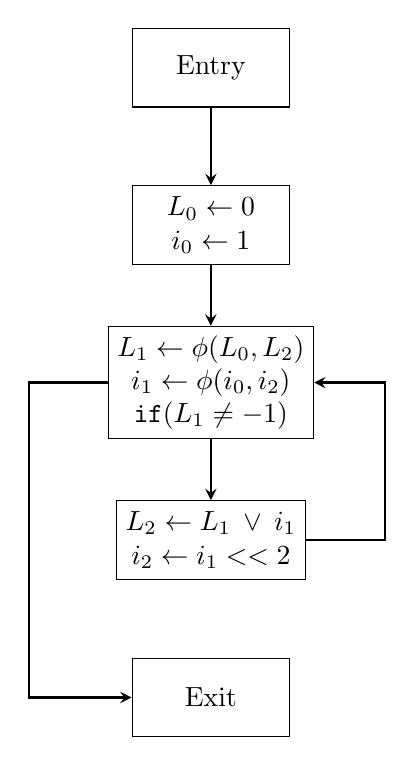
\begin{tikzpicture}
        \tikzstyle{node} = [rectangle, minimum width=2cm, minimum height=1cm, text centered, draw=black, node distance=2cm]
        \tikzstyle{arrow} = [thick,->,>=stealth]
                
                \node (entry) [node, xshift=1cm] {Entry};
                \node (b1) [node, below of=entry, align=center] {$L_0 \leftarrow 0$\\$i_0 \leftarrow 1$};
                \node (b2) [node, below of=b1, align=center] {$L_1 \leftarrow \phi(L_0, L_2)$ \\ $i_1 \leftarrow \phi(i_0, i_2)$\\ $\mathtt{if} (L_1 \neq -1)$};
                \node (b3) [node, below of=b2, align=center] {$L_2 \leftarrow L_1 \: \lor \: i_1$ \\ $i_2 \leftarrow i_1 << 2$};
                \node (exit) [node, below of=b3] {Exit};
                
                \draw[arrow] (entry) -- (b1);
                \draw[arrow] (b1) -- (b2);
                \draw[arrow] (b2) -- (b3);
                \draw[arrow] (b3.east) -- ++(1,0) |- (b2.east);
                \draw[arrow] (b2.west) -- ++(-1,0) |-(exit.west);
    \end{tikzpicture}
    \caption{CFG of the example program}\label{fig:loopEx}
    \label{fig:whilegraph}
\end{subfigure}
\caption{Example program for Loop Analysis. The program doesn't have a secret input and always returns $-1$.}
\end{figure}

\paragraph{General Loop Body Analysis}
We begin the analysis by defining input and output values for a single loop iteration. 

The set of values that are used inside a loop can be divided into two categories:
\begin{enumerate}
    \item Values, that might change with each iteration. These are values that are defined inside the loop (or before the loop in the case of the first loop iteration) and then get passed to the next iteration via a $\phi$-function in the loop head.
    \item Values, that are constant for every loop iteration.
\end{enumerate}

The first group of values represent the inputs of a loop iteration, while the second group can be treated as constants in the loop analysis, even if their concrete value is unknown. The outputs of a loop iteration are the values that are defined inside the loop and used either in the subsequent iteration or after the loop.

\begin{definition}[Loop Inputs and Outputs]
    Let $l$ be a loop in program $p$.
    \begin{itemize}
        \item[(a)] We define the set $in[l]$ of inputs of the loop as the set of values defined by $\phi$-functions in $l$.
        \item[(b)] We define the set $out[l]$ of outputs of the loop as the set of values that are defined inside the loop \emph{and} appear as arguments in a $\phi$-function in $l$.
    \end{itemize}
\end{definition}

Analogous to the notation for values, $in[l]$ and $out[l]$ refer to the input and output sets during the general loop body analysis. The in- and outputs for a specific iteration $i$ are then called $in[l(i)]$ and $out[l(i)]$.

Using the defined inputs and outputs, we can apply the principles of the dependency analysis for linear programs to the loop $l$:

We set $dVec(v[l]) = \var(v[l])$ for $v[l] \in in[l]$, i.e. we represent the values of the inputs as vectors of fresh boolean variables.

Next, we compute the dependency vectors of all values defined inside the loop. To do that we analyse the blocks $l$ in topological order.

The dependency vectors of the loop outputs $out[l]$ are made up of formulas that depend on
\begin{enumerate}
    \setlength\itemsep{0em}
    \item Variables that represent loop input bits
    \item Variables that represent program input bits
\end{enumerate}

Additional to the inputs and outputs, we define a propositional formula $exit[l]$ for the $l$, that represents the condition that must be fulfilled to jump out of the loop. The  condition $exit[l]$ is given by the condition $follow(e)$ that belongs to the edge $e$ that connects the loop header of $l$ to its outside-loop successor. Like the formulas for values in $out[l]$, $exit_l$ depends on variables from the loop inputs as well as the program inputs. 

\paragraph{Example}
Figure \ref{fig:loopEx} shows an example of a program containing a loop $l$.

The inputs of the loop are the values $L_1[l]$ and $i_1[l]$. The outputs of the loop are the values $L_2[l]$ and $i_2[l]$.

The dependency vectors of those values are:
\begin{align*}
    dVec(L_1[l]) &= [L_1^2, L_1^1, L_1^0] \\
    dVec(i_1[l]) &= [i_1^2, i_1^1, i_1^0] \\
    dVec(L_2[l]) &= [L_1^2 \lor i_1^2, L_1^1 \lor i_1^1, L_1^0 \lor i_1^0] \\
    dVec(i_2[l]) &= [i_1^1, i_1^0, 0] \\
\end{align*}

The loop condition is $enter_l = (L_1[l] \neq -1)$.

\paragraph{Computing Iterations}
In the previous paragraph, we computed dependency vectors that represent the output values of the loop using abstract values as the inputs.

In this paragraph, we use this general result, to obtain dependency vectors that represent the loop outputs after a specific iteration. The formulas in these vectors will then only depend on the program input variables and not the loop variables.

Input and output values of specific loop iterations are collected in the sets $in[l(i)]$ and $out[l(i)]$, where $i$ is the iteration count. The special case $i = 0$ refers to the program state before the loop is entered. Here we define $in[l(0)]$ as $\emptyset$ and $out[l(0)]$ as the values that computed before the loop and then used inside the loop during the first iteration. For $i > 0$ we have $out[l(i)] = in[l(i + 1)]$.

Given the dependency vectors for values in $in[l(i)]$ for some value of $i$, we can compute the dependency vectors for values in $out[l(i)]$, by substituting the variables representing values in $in[l]$ by the corresponding formula of the value in $in[l(i)]$.

\begin{definition}[Iteration Substitution]
    Let $p$ be a program with a loop starting at block $l$. We are given dependency vectors for values in $in[l(i)]$. To compute the dependency vectors for values in $out[l(i)]$, we use the substitution
    \begin{center}
        $\sigma_{l(i)} := \{h_i^j \mapsto dVec(h_i)^j | \quad h_i \in in[l(i)]\}$
    \end{center}
    and apply it to the dependency vectors of $out[l]$.
\end{definition}

The substitution $\sigma_{l(i)}$ can be applied to $exit[l]$ to obtain a formula $exit[l(i)]$ that represents the condition of whether the i-th loop iteration will be entered or not.

\paragraph{Example (cont'd)} The dependency vectors of the input and output values, as well as the loop condition, for the first iterations for the example program are presented in table \ref{tab:loop}.

\begin{table}
    \centering
    \begin{tabular}{|c|c|c|c|c|c|}
    Iteration & \multicolumn{2}{|c|}{Inputs} & \multicolumn{2}{|c|}{Outputs} & Exit Condition \\
     & $L_1[l(i)]$ & $i_1[l(i)]$ & $L_2[l(i)]$ & $i_2[l(i)]$ & $exit[l(i)]$ \\
     \hline
     $i = 0$ & - & - & $[0 0 0]$ & $[0 0 1]$ & $[000] == [111]$ \\
     $i = 1$ & $[0 0 0]$ & $[0 0 1]$ & $[0 0 1]$ & $[0 1 0]$ & $[001] == [111]$ \\
     $i = 2$ & $[0 0 1]$ & $[0 1 0]$ & $[0 1 1]$ & $[1 0 0]$ & $[011] == [111]$ \\
     $i = 3$ & $[0 1 1]$ & $[1 0 0]$ & $[1 1 1]$ & $[0 0 0]$ & $[111] == [111]$ \\
    \end{tabular}
    \caption{Dependency Vectors for the values of the sets $in[l(i)]$ and $out[l(i)]$ for the example program \ref{fig:whilegraph}.}
    \label{tab:loop}
\end{table}

\paragraph{Combining Iterations for Overall Loop Result}
To finish the loop analysis, we compute dependency vectors for the output values, that represent the loop execution as a whole.

The result values of the loop depend on the number of iterations that are executed. The case that the loop is executed exactly $i$ times is represented by the condition $upto[l(i)]$:

\begin{definition}[Loop Iterations]
    Let $p$ be a program with a loop beginning with basic block $l$.
    The propositional formula
    \begin{center}
        $upto[l(i)]: (\bigwedge\limits_{0 \leq j < i} \lnot exit[l(j)]) \land exit[l(i)]$
    \end{center}
    is a propositional formula over $\var_p$ and evaluates to true, iff for a program input $h$ the loop is executed exactly $i$ times.
\end{definition}

The formula $upto[l(i)]$ encodes the following intuition: For every $j < i$, $exit[l(j)]$ must be false, otherwise the loop execution would have been aborted before the $i$-th iteration. The condition $exit[l(i)])$ must be true, otherwise the loop would have been executed more than $i$ times.

For the final set of loop output values, we make the following observations:

If the loop is executed exactly $i$ times, the results are equal to the outputs $out[l(i)]$. Whether the loop is executed exactly $i$ times or not, can be checked via the condition $upto[l(i)]$. Continuing this observation for more iterations, leads to the algorithm \ref{alg:loop} that computes the dependency vector for a loop output value.

\begin{algorithm}
    \hspace*{\algorithmicindent} \textbf{Input} Iteration results $v[l(i)]$ for the loop output value $v$ and \\
    \hspace*{\algorithmicindent} iteration conditions $upto[l(i)]$ \\
    \hspace*{\algorithmicindent} \textbf{Output} $dVec(v):$ Dependency vector that represents the overall computation result\\
    \hspace*{\algorithmicindent} \hspace*{\algorithmicindent}of the loop for the value $v$. \\
    \begin{algorithmic}[1]
        \State $dVec(v) \leftarrow \bot$ // initialize with placeholder value
        \State $i: int \leftarrow 0$
        \While{$\mttt$}
            \State $dVec(v) \leftarrow dVec(v).replace(\bot, \mathbb{IF}(iterate(i), \: dVec(v[i]), \bot))$
        \EndWhile
        \State The function \texttt{o.replace(x, y))} replaces each occurrence of \texttt{x} in the expression \texttt{o} by \texttt{y}
        \end{algorithmic} 
\caption{Loop Result Computation}\label{alg:loop}
\end{algorithm}

\paragraph{Approximation: Limiting Loop Iterations}
Algorithm \ref{alg:loop} is correct but doesn't terminate. To terminate the algorithm, we have to limit the number of loop iterations it computes to an upper bound $loopMax$, by replacing the condition in the while loop with $i < loopMax$.
Limiting the number of loop iterations means, that we exclude certain program inputs $h$ from the analysis, namely those that need more than $loopMax$ iterations. If such an input is used to evaluate the dependency vector of a loop output value $v$, $dVec(v)$ will evaluate to $\bot$. We interpret $\bot$ as an invalid execution and disregard the value in the following analysis.

The exclusion of certain input values means, we have to adjust the equivalence from theorem \ref{thm:equiv}:

\begin{theorem}[Weakened Equivalence Theorem]\label{thm:weak}
    Given a program $p$ and a program input value $h$, the dependency vector of a value $v$ fulfills the following condition:
    \begin{center}
        $\forall 0 \leq i < w: \mathcal{V}_h(dVec(v)^i) \implies \llbracket p \rrbracket_h (v)^i$
    \end{center}
\end{theorem}

Let $p$ be a program that contains a loop. We consider an execution that produces the output value $l$. We analyse the indistinguishability set of the execution using the formula $F_{dyn}$ as defined in \ref{lemma:dyn}, however, the dependency vectors used in the formula contain the approximation described above. The indistinguishability set will therefore also be an approximation. To differentiate this from the exact result, we write $\mathcal{H}_l^{approx}$
From theorem \ref{thm:weak} follows that, every model that fulfills the condition $F_{dyn}$, still induces an input value $h$, whose execution will result in the output $l$. Therefore the input value $h$ is an element of $\mathcal{H}_l$. On the other hand, there might be input values $h'$, whose execution would produce the output $l$, but who are not identified as a model of $F_{dyn}$ because the execution would need more than $loopMax$ iterations and is therefore regarded as invalid.
Therefore $\mathcal{H}_l^{approx} \subseteq \mathcal{H}_l$ and $|\mathcal{H}_l^{approx}| < |\mathcal{H}_l|$, i.e. we under-approximate the size of $\mathcal{H}_l$. Under-approximation is sound, because the knowledge gained by the attacker increases as the size of $\mathcal{H}_l$ decreases. Therefore the approximated dynamic leakage is a safe upper bound for the information leaked by the execution.


\paragraph{Example (cont'd)}
Applying algorithm \ref{alg:loop} to the values $L_2$ and $i_2$ from example \ref{fig:whilegraph}, gives the following results:
\begin{center}
\td{complete example}
\end{center}

\section{Functions}
We assume that all functions that are part of the input program are pure, i.e. they have no side effects. This means, the only way for information to flow into and out of the function is through the input parameters and the return value.

We write $\func$ for the set of functions that belong to a program $p$ and for $f \in \func$. For the analysis of the function $f$, we treat $f$ as its own program, where the parameters correspond to the input $\mIn$ and the return value corresponds the output $\mOut$.

\paragraph{Function Analysis}
In this paragraph we only consider the analysis of non-recursive functions with a single return statement. Independent of any call sites of the function, we use the standard dependency analysis algorithm to compute dependency vectors for all values inside the function.

The dependency vectors computed for values of this function are defined over the variables created to represent the function's parameters. They do not contain variables representing bits of values from outside the function.


%\begin{definition}[Value Selection Function]
%    Let $f$ be a function and $V := \{v_0,..., v_n \} \subseteq \val_p$ be a set of values that, where $\forall v_i \neq v_j \in V: exec(def(v_i)) \land exec(def(v_j))$. We define the function $select: 2^{\val_f} \to \mbform^w $ as
%    \begin{center}
%        $select(r_0, ..., r_n) := \begin{cases}
%            \mathbb{IF}(exec(def(r_0)), \: dVec(r_0), \: dVec(r_1)) & \text{if $n = 1$}, \\
%            \mathbb{IF}(exec(def(r_0)), \: dVec(r_0), \: select(r_1,...,r_n)) & \text{otherwise}
%        \end{cases}$
%    \end{center}
%\end{definition}

%\begin{lemma}[Combining Dependency Vectors based on Control Flow]
%    Let $f$ be a function and $V := \{v_0,...v_n \} \subseteq \val_p$ be a set of values that could possibly be returned by $f$
%    Then the return dependency vector of $f$ is given by
%    \begin{center}
%        $return(f) = select(r_0, ..., r_n)$
%    \end{center}
%\end{lemma}

\paragraph{Dependency Analysis for \texttt{call}-Statements}
The statement $v \leftarrow \mathtt{call} f(a)$ calls the function $f$ with the arguments $a := (a_0,..., a_m)$ and assigns the return value of the call to the value $v$. To compute the dependency vector $dVec(v)$, we substitute the variables in $\var_f$ with the dependency vectors of the arguments:

\begin{definition}[Callsite Substitution]
    Let $f \in \func$ be a function in $p$ that has input parameters $\mathtt{P} := (\mathtt{P}_0,...,\mathtt{P}_m)$ and let the expression $\mathtt{call} f(a)$ be a call to $f$ with the arguments $a := (a_0,..., a_m)$.
    
    The substitution $\sigma_{f(a)}$, defined as
    \begin{center}
        $\sigma_{f(a)} := \{ \var(\mathtt{P}_i)^j \mapsto dVec(a_i)^j \: |  \mathtt{P}_i \in \mathtt{P}\}$
    \end{center}
    is called the \emph{callsite substitution} of the expr $\mathtt{call} \: f(a)$ and substitutes the variables $\var(\mathtt{P}_i)$ representing the input parameters $\mathtt{P}_i$ by the corresponding boolean predicates of the dependency vectors belonging to the callsite's arguments.
    The definition of $\mathcal{E}: \expr \to \mbform$ for function call expressions is then given as:
    \begin{center}
        $\mathcal{E}(\mathtt{call} f(a)) := \sigma_{f(a)} (dVec(r_f))$
    \end{center}
\end{definition}

\begin{lemma}
Using the extended definition of $\mathcal{E}$ including call-expressions, theorem \ref{thm:equiv} (theorem \ref{thm:weak} in case of loop approximation) is still fulfilled.
\end{lemma}

\section{Recursion}

\section{Break-Statements}

\section{Arrays}
The analysis can support fixed-size arrays. For fixed-size arrays, the length must be known at the time of instantiation.